       
\chapter{Systemarchitektur}
\section{Einführung}
In diesem Kapitel wird die Systemarchitektur der Anwendung vorgestellt, indem erläutert wird wie die verschiedenen Komponenten und Technologien zusammenarbeiten und miteinander kommunizieren.
Die Anwendung ist in zwei Hauptkomponenten unterteilt: das Frontend und das Backend. Das Frontend ist für die Darstellung der Benutzeroberfläche und die Interaktion mit dem Benutzer verantwortlich, während das Backend die Spiellogik, die Verwaltung der Benutzerdaten und die Echtzeit-Kommunikation zwischen den Spielern steuert.

Die Anwendung verwendet moderne Web-Technologien, um eine reaktive und benutzerfreundliche Oberfläche zu schaffen. Das Frontend basiert auf dem React-Framework\footcite{react}, das es ermöglicht, wiederverwendbare Komponenten zu entwickeln und den Anwendungsstatus effizient zu verwalten. Das User-Interface basiert auf Chakra UI\footcite{chakraui}, einem modernen und flexiblen Komponenten-Bibliothekssystem, das die Entwicklung von responsiven und zugänglichen Benutzeroberflächen erleichtert. Die Benutzerführung und die Kommunikation zwischen den React-Komponenten sind so gestaltet, dass sie eine nahtlose und intuitive Benutzererfahrung bieten.

Auf der Backend-Seite wird Node.js\footcite{nodejs} mit dem Express-Framework verwendet, um einen leistungsstarken und skalierbaren Server bereitzustellen. Die API-Endpunkte und die Echtzeitkommunikation mittels Socket.io ist so konzipiert, dass sie den Anforderungen der verschiedenen Frontend-Komponenten gerecht werden und die Kommunikation zwischen Frontend und Backend erleichtern. Für die Speicherung und Verwaltung der Benutzerdaten zum Anmelden wird eine PostgreSQL\footcite{postgresql}-Datenbank verwendet, die aufgrund ihrer Leistungsfähigkeit und Flexibilität ausgewählt wurde. Freundeslisten und Daten aktiver Spiele werden in einer Redis\footcite{redis}-Datenbank gespeichert, die sich durch hohe Leistung und niedrige Latenz auszeichnet, insbesondere bei Lese- und Schreibvorgängen. Redis, eine In-Memory-Datenstruktur, eignet sich ideal für Anwendungen, bei denen schnelle Zugriffszeiten und Skalierbarkeit wichtig sind. Die Kombination von PostgreSQL und Redis ermöglicht eine effiziente Verwaltung sowohl persistenter als auch flüchtiger Daten und fördert eine optimale Benutzererfahrung.
\section{Architekturübersicht}
Das Komponentendiagramm in Abbildung \ref{fig:Komponentendiagramm} visualisiert die Hauptkomponenten und deren Schnittstellen der Kommunikation.

Im Frontend gibt es drei Komponenten, welche die Web-API verwenden: Der \textit{UserContext}, \textit{Login} und \textit{SignUp}. Unsere Web-API verwendet dabei nur die Methoden GET und POST. Der \textit{UserContext} ist verantwortlich für die Verwaltung des Benutzerzustands, während die Komponenten \textit{Login} und \textit{SignUp} das setzen des Benutzerzustands über das Anmelden und Registrieren unterstützen. Der \textit{SocketContext} baut die Socket.io Verbindung für die Echtzeitkommunikation auf und stellt sie den restlichen React Komponenten zur Verfügung, um Events zu senden und zu empfangen.

Die Anfragen über die Web-API werden durch den in \textit{authRouter} definierten Express Router entgegengenommen. Zur Behandlung werden in ihm verschieden Middlewares der Datei \textit{authController} für verschiedene Anfragen festgelegt, welche auf die PostgreSQL Datenbank zugreifen. Die Web-API und die PostgreSQL Datenbank werden lediglich für das Registrieren und Anmelden von Benutzern verwendet.

Beim Herstellen einer Socket.io Verbindung in \textit{SocketContext} werden im Backend die Middlewares aus \textit{socketMiddleware} ausgeführt, welche unter anderem die Listener aus \textit{socketController} und \textit{socketChessContoller} initialisieren. Der Unterschied zwischen den Listenern aus den beiden Dateien ist dabei, dass \textit{socketController} sich um allgemeine Funktionen wie das Versenden von Freundschaftsanfragen oder das senden von Informationen an das Frontend kümmert, während \textit{socketChessController} Listener enthält, welche sich um Funktionen des Schachspiels kümmert, wie zum Beispiel das Behandeln eines neuen Zugs. 

Alle Dateien im sockets Package verwenden den \textit{redisController}, um Daten aus der Redis Datenbank abzurufen und zu speichern. Beispielsweise werden Freundschaftsanfragen, Freunde und Daten aktiver Spiele in der Redis Datenbank von dem \textit{redisController} verwaltet, abgerufen und gespeichert.

\begin{figure}[h!]
\centering
\begin{tikzpicture}
 \begin{umlpackage}[x=4]{Frontend}
 \begin{umlcomponent}{UserContext}
 \begin{umlcomponent}{SocketContext}
 \umlbasiccomponent{Login}
 \umlbasiccomponent[x=3]{SignUp}
 \end{umlcomponent}
 \end{umlcomponent}
 \end{umlpackage}
 
 
 \begin{umlpackage}[y=-5]{Backend}
 \begin{umlpackage}{sockets}
 \umlbasiccomponent{socketController}
 \umlbasiccomponent[x=5]{socketChessController}
 \umlbasiccomponent[x=2.5, y=-2.5]{socketMiddleware}
 \end{umlpackage}
 \umlbasiccomponent[x=2.5, y=-5]{redisController}
 \umlbasiccomponent[x=10]{authRouter}
 \umlbasiccomponent[x=10, y=-5]{authController}
 \end{umlpackage}
 
\umlHVassemblyconnector[with port, anchor2=130]{SocketContext}{sockets}

\umlHVassemblyconnector[with port]{UserContext}{authRouter}
\umlVHVassemblyconnector[with port, anchor1=-90]{Login}{authRouter}
\umlVHVassemblyconnector[with port, anchor1=-90]{SignUp}{authRouter}

\umlnote[x=-1,y=2]{SocketContext-west-port}{socket.io-client}
\umlnote[x=12, y=2]{UserContext-east-port}{Web-API}
\umlnote[x=12, y=-1]{authRouter-north-port}{Express Router}
 
 \umlbasiccomponent[x=2.5, y=-13]{Redis DB}
 \umlbasiccomponent[x=10, y=-13]{PostgreSQL DB}
 
\umlassemblyconnector[anchor1=-90, anchor2=90]{authRouter}{authController} 
\umlVHassemblyconnector[anchor1=-90, anchor2=-180]{socketController}{redisController}
\umlVHassemblyconnector[anchor1=-90, anchor2=0]{socketChessController}{redisController}
\umlVHassemblyconnector[anchor1=-90, anchor2=90]{socketMiddleware}{redisController}

 
 \umlassemblyconnector[with port, anchor1=-90, anchor2=90]{authController}{PostgreSQL DB}
  \umlassemblyconnector[with port, anchor1=-90, anchor2=90]{redisController}{Redis DB}
\end{tikzpicture}
\caption{Komponentendiagramm der Anwenundung}
\label{fig:Komponentendiagramm}
\end{figure}

\section{Konzept der Schachuhren}
Bei der Konzeption der Schachuhren war ein Aspekt besonders entscheidend: Was passiert, falls ein Spieler vorübergehend keine Internetverbindung beim senden oder beim empfangen hat?

Um den Server zu entlasten wäre natürlich eine Client basierte Lösung ideal, bei der mit einem Zug auch die jeweilige aktuelle Zeit gesendet wird. Wenn ein Spieler allerdings eine schlechte Internetverbindung hat und deshalb der Zug im Backend und bei dem anderen Spieler erst später ankommt können sich die Zeiten der beiden Spieler erheblich unterscheiden. Es stellt sich die Frage, welche dieser Zeiten jetzt gültig ist. Trivialerweise entsteht das gleiche Problem bei einer verzögerten Zustellung. Wenn die Zeit auf einem Client bereits abgelaufen wäre, könnte sie auf dem anderen noch weiterlaufen. Hat der Spieler dann gewonnen oder nicht?

Um dieses Problem zu umgehen liegt die einfachste Lösung darin, eine serverseitige Schachuhr einzuführen. Diese Uhr bestimmt die aktuellen Zeiten. Wenn ein Zug im Backend ankommt, wird die auf dem Server gültige Zeit an die Clients gesendet. Dadurch gibt es keine Unklarheiten hinsichtlich der aktuellen Zeit. Wenn eine Zeit auf dem Server abläuft wird dies durch ein Event mitgeteilt.  Es kann zwar vorkommen, dass bei den Clients zu dem Zeitpunkt noch Zeit übrig ist, wenn das letzte Event aufgrund einer schlechten Verbindung verspätet eingetroffen ist, aber dieses Problem ist unvermeidbar.

Durch dieses Konzept umgeht man auch das Problem, dass Client seitiger Code im Browser manipulierbar sein kann und dadurch die Schachuhren beeinflussbar wären.

Wie die Schachuhren konkret funktionieren wird in den nachfolgenden Kapiteln behandelt.

    \section{Frontend-Architektur}
Das Frontend der Anwendung wurde unter Verwendung von React (Abschnitt \ref{sec:react}), Socket.io (Abschnitt \ref{sec:socket.io}) und weiteren Bibliotheken aus Abschnitt \ref{sec:weiteres} entwickelt.

\begin{figure}[h!]
\centering

\begin{minipage}{0.6\textwidth}
\dirtree{%
.1 client/.
.2 public/.
.3 Gambit dark.png.
.3 Gambit light.png.
.3 Gambit springer.png.
.3 index.html.
.3 manifest.json.
.3 robots.txt.
.2 src/.
.3 components/.
.4 ActiveGames.js.
.4 AddFriendModal.js.
.4 Chat.js.
.4 ChessClock.js.
.4 Friend.js.
.4 FriendList.js.
.4 FriendRequest.js.
.4 GameRequests.js.
.4 Navbar.js.
.4 PromotionModal.js.
.3 contexts/.
.4 AccountContext.js.
.4 SocketContext.js.
.4 tests/.
.3 themes/.
.4 Theme.js.
.3 utils/.
.4 ChessLogic.js.
.3 views/.
.4 ChessGame.js.
.4 Home.js.
.4 Login.js.
.4 Signup.js.
.3 App.js.
.3 index.js.
.3 Views.js.
.2 package.json.
}
\end{minipage}
\caption{Ordnerstruktur des Frontends}
\label{fig:frontend_dirtree}

\end{figure}

Die Ordnerstruktur (Abbildung \ref{fig:frontend_dirtree}) ist wie folgt aufgebaut:
\begin{itemize}
\item \textbf{public:} In diesem Ordner befinden sich statische Ressourcen, wie zum Beispiel Bilder des Logos, die von der Anwendung verwendet werden.
\item \textbf{components:} Dieser Ordner enthält alle React-Komponenten, die für die Anwendung verwendet werden. Sie sind modular und stellen jeweils nur ein Teil eines User Interfaces dar.
\item \textbf{contexts:} Hier befinden sich die React Contexts, die zum Verwalten von globalen Zuständen und Kommunikationsschnittstellen verwendet werden.
\item \textbf{themes:} Dieser Ordner enthält Dateien, die für das Design und die Anpassung des Aussehens der Anwendung mittels Chakra UI verantwortlich sind.
\item \textbf{utils:} In diesem Ordner befinden sich Hilfsdateien, die ausgelagerte Funktionen zur Verfügung stellen.
\item \textbf{views:} Dieser Ordner enthält die verschiedenen Seiten der Anwendung. Zu diese Seiten kann mit Hilfe des React-Routers über verschiedene Pfade navigiert werden. Diese Seiten verwenden teilweise die Komponenten aus dem components-Ordner, um eine vollständige Benutzeroberfläche darzustellen.
\end{itemize}
    
        \subsection{React-Komponenten}
Der hierarchische Aufbau der React-Komponenten in Abbildung \ref{fig:frontend_tikz} zeigt die Struktur und Verschachtelung der Anwendung für angemeldete Benutzer. Nicht angemeldete Benutzer sehen lediglich die Komponenten ActiveGames und FriendList nicht, während der restliche Aufbau gleich bleibt. In diesem Abschnitt werden die wichtigsten Komponenten und ihre Funktionen innerhalb der Anwendung erläutert.
        
\begin{itemize}
\item \textbf{AccountContext:} Stellt Informationen über den Benutzerstatus allen Folgenden Komponenten mittels eines Contexts zur Verfügung. Diese Informationen beinhalten, ob ein Benutzer angemeldet ist und falls er das ist seinen Benutzernamen.
\item \textbf{SocketContext:} In diesem React Context wird eine socket.io Verbindung mit dem Server hergestellt und allen darauf folgenden Komponenten bereitgestellt.
\item \textbf{ChakraBaseProvider und ColorModeScript:} Diese importierten Komponenten von ChakraUI stellen die Funktionen zum designen bereit. Dazu gehören Beispielsweise das Verwenden des globalen Zustands des Farbenschemas (dunkel oder hell) oder das zugreifen auf definierte Stile.
\item \textbf{Views:} Diese Komponente beinhaltet das User Interface. Mit Hilfe des React-Routers werden hier die Komponenten des \verb|view|-Ordners unter einem bestimmten Pfad definiert. Des weiteren beinhaltet es die Komponenten GameRequest und Navbar, welche durch die Definition in dieser Komponente auf jedem Pfad vorhanden sind.
\begin{itemize}
\item \textbf{Navbar:} Die Navigationsleiste besteht aus dem Logo und einem Button zum wechseln des Farbschemas. Je nachdem, ob ein Benutzer angemeldet ist oder nicht beinhaltet es noch Buttons zum Anmelden, Registrieren oder Abmelden (siehe Abbildungen \ref{fig:home-not-logged-in} \& \ref{fig:home-logged-in}).
\item \textbf{GameRequests:} Diese Komponente ist dafür Verantwortlich beim Eingang einer Spielanfrage eines Freundes, dieses als Modal darzustellen und bietet die Möglichkeit diese Anfrage zu beantworten (siehe Abbildung \ref{fig:game-request}).
\end{itemize}
\item \textbf{Home:} Diese Komponente stellt die Startseite dar und enthält die Buttons zum Starten eines Spiels mit verschiedenen Schachuhr Konfigurationen (siehe Abbildung \ref{fig:home-not-logged-in}). Ist ein Benutzer angemeldet sind auch noch die Komponenten ActiveGames und FriendList auf der rechten Seite vorhanden (siehe Abbildung \ref{fig:home-logged-in}).
\begin{itemize}
\item \textbf{ActiveGames:} ActiveGames ist eine Komponente die alle derzeit aktiven Spiele mit den Informationen der Benutzernamen und wer welche Farbe spielt als Buttons darstellt (siehe Abbildung \ref{fig:home-logged-in}). Beim klicken auf einen dieser Buttons wird zu der aktiven Partie navigiert.
\item \textbf{FriendList:} Diese Komponente verwaltet alle Freunde und Freundschaftsanfragen eines Benutzers, während die Darstellung die Unterkomponenten Friend und FriendRequest übernehmen.
\begin{itemize}
\item \textbf{Friend:} Übernimmt die Darstellung eines Freundes. Mittels eines farbigen Punktes ist erkennbar, ob dieser Freund gerade online ist (grün) oder nicht (rot) (siehe Abbildung \ref{fig:home-logged-in}). Ist er online erscheint noch mindestens ein weiterer Button. Es beinhaltet ein Icon in Form von gekreuzten Schwertern und einem Schild. Dies hat die Funktion einen Freund zu einem Spiel herauszufordern. Falls dieser Freund gerade ein aktives Spiel hat erscheint noch ein zweiter Button mit einem Auge als Icon, welches den Benutzer zu dem aktiven Spiel des Freundes als Zuschauer navigiert.//Bilder
\item \textbf{FriendRequest:} Eine Freundschaftsanfrage wird mittels dieser Komponente dargestellt und beantwortet (siehe Abbildung \ref{fig:home-logged-in}).
\item \textbf{AddFriendModal:} Mit Hilfe dieser Komponente können Freundschaftsanfragen unter Angabe des Benutzernamens versendet werden. // BILD
\end{itemize}
\end{itemize}

\item \textbf{Login \& SignUp:} Komponenten, die das Anmelden und Registrieren mittels Formularen mit Formik und Yup (siehe Abschnitt \ref{sec:formik}) ermöglichen und mit dem Server zur Authentifizierung kommunizieren. //BILD
\item \textbf{ChessGame:} Die Komponente ChessGame ist das Herzstück der Anwendung, da dort das eigentliche Schachspiel stattfindet. Die ChessGame Komponente wird durch den Pfad \verb|/game/:roomId| gerendert und holt sich durch die roomId die Spieldaten vom Backend (siehe Abschnitt \ref{sec:game-suche} für eine detaillierte Beschreibung des Ablaufs beim Starten / Suchen eines Spiels) . In der Abbildung \ref{fig:chess-game} ist eine beispielhafte Komponente zu sehen. Auf der rechten Seite neben dem Brett befindet sich die \textit{ChessClock} Komponete und daneben befindet sich die \textit{Chat} Komponente. Das Spielfeld und die Figuren entstehen durch die Bibliothek chessground, während die Spiellogik hinter dem Schachspiel von chess.js verwaltet wird (siehe Abschnitt \ref{sec:chess.js}). Eine dataillierte Beschreibung, was in der Komponente beim spielen oder empfangen eines Zuges passiert befindet sich im Abschnitt \ref{sec:Schachspiel}.



\begin{itemize}
\item \textbf{ChessClock:} ChessClock ist eine Komponente, die die Verwaltung und Darstellung der Schachuhren übernimmt.
\item \textbf{Chat:} Die Chat Komponente repräsentiert einen simplen gehaltenen Chat in dem die beiden Spieler kommunizieren können. Zuschauer können ihn lesen, allerdings nichts selber schreiben, da sie Tipps geben könnten.
\end{itemize}
\end{itemize}
 
\begin{figure}[h!]
        \centering
        \begin{tikzpicture}
\node {App}
    child {node {AccountContext}
    		child {node {SocketContext}
    			child {node {ChakraBaseProvider} [sibling distance = 2.5cm]
    				child {node [xshift= -2cm] {ColorModeScript}}
    					child {node {Views} [sibling distance = 2.6cm]
    						child {node {Home} edge from parent [dashed]					
    							child {node {ActiveGames} edge from parent [solid]}
    							child {node {FriendList} [sibling distance = 2.0cm] edge from parent [solid]
								child {node {Friend}}
    								child {node {...}}
    								child {node {FriendRequest}}
    								child {node {...}}
    								child {node {AddFriendModal}}    							
    							 }
    						}
    						child {node {Login} edge from parent [dashed]}  
    						child {node {SignUp} edge from parent [dashed]}  				
    						child {node {ChessGame} edge from parent [dashed]
						child {node {ChessClock} edge from parent [solid]}
						child {node {Chat} edge from parent [solid]}    						
    						}
						child {node {GameRequests}}
						child {node {Navbar}}  
    					}
    				} 
    			}
    		};
    		

    \node[anchor=north east, xshift=-7cm] (dashed) at (current bounding box.north east) {};
    \draw[dashed] (dashed.east) -- ++(0.8cm, 0);

    \node[anchor=west, right=1cm of dashed] {Route Komponenten};

    \node[below=0.3cm of dashed] (solid) {};
    \draw[solid] (solid.east) -- ++(0.8cm, 0);

    \node[anchor=west, right=1cm of solid] {enthaltene Unterkomponenten};
\end{tikzpicture}
    	
\caption{Aufbau der React-Komponenten für angemeldete Benutzer}
\label{fig:frontend_tikz}
        
        \end{figure}

  \begin{figure}[htbp]
  \centering
  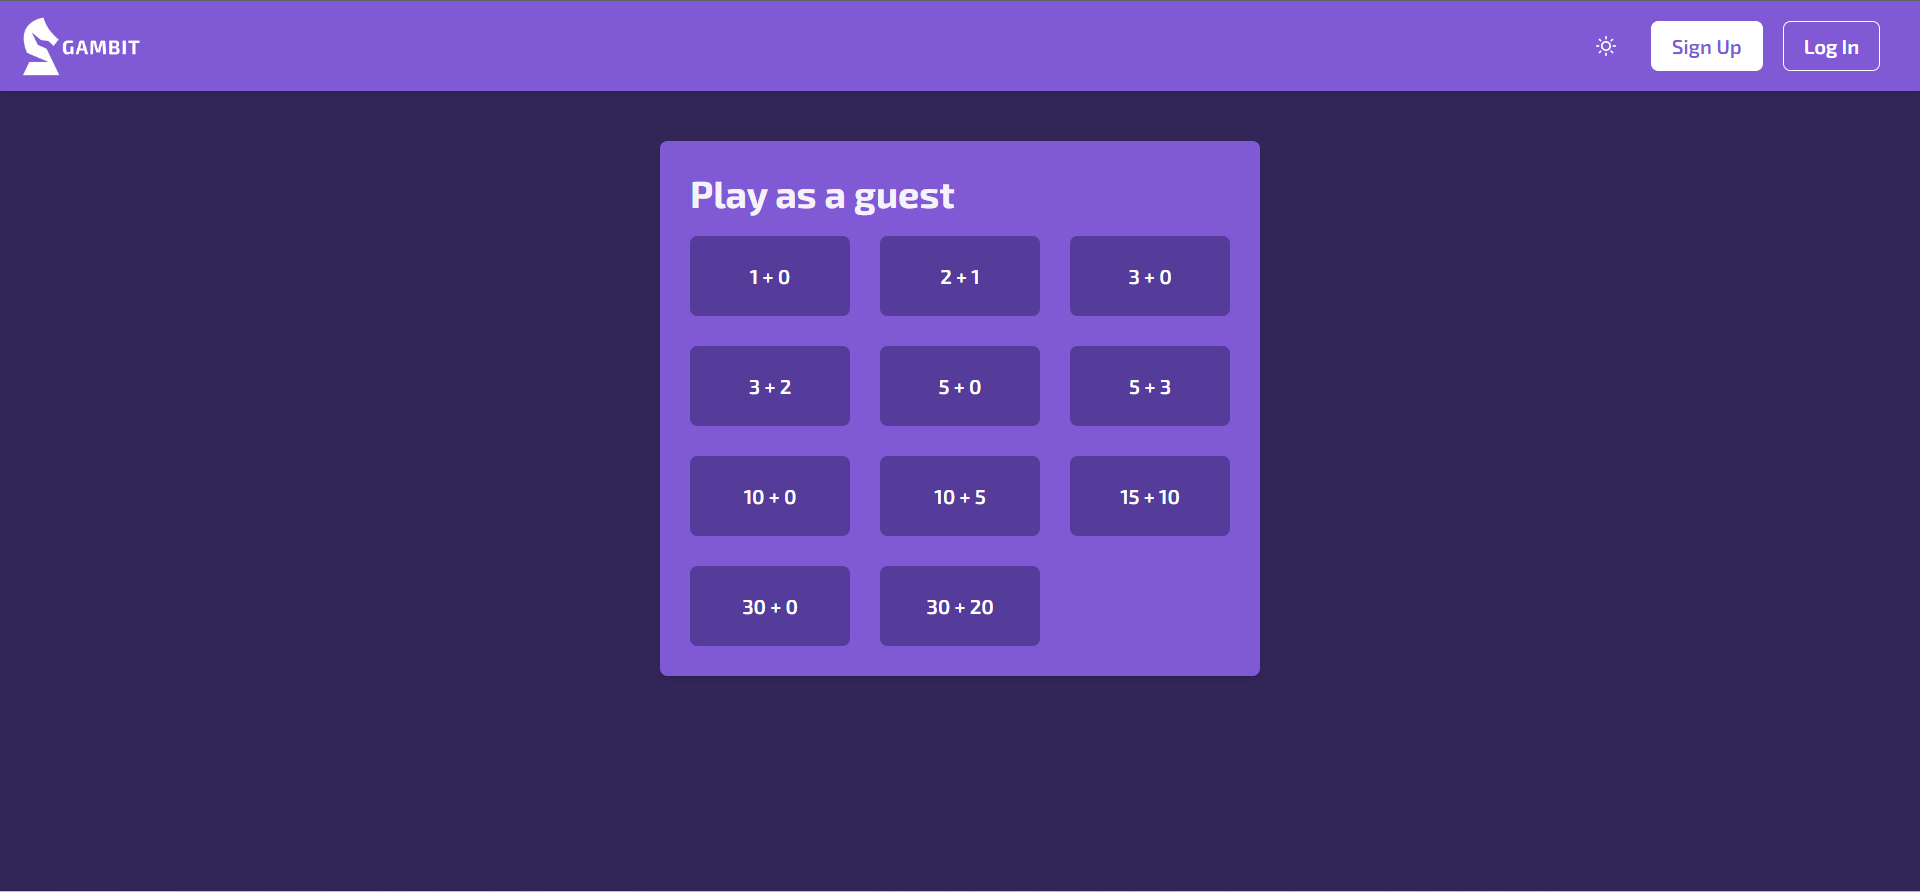
\includegraphics[width=160mm]{Home_not_logged_in.png}
  \caption{Home und Navbar Komponente eines nicht angemeldeten Benutzers im dunklen Farbschema}
  \label{fig:home-not-logged-in}
\end{figure}

  
    \begin{figure}[htbp]
    \centering
  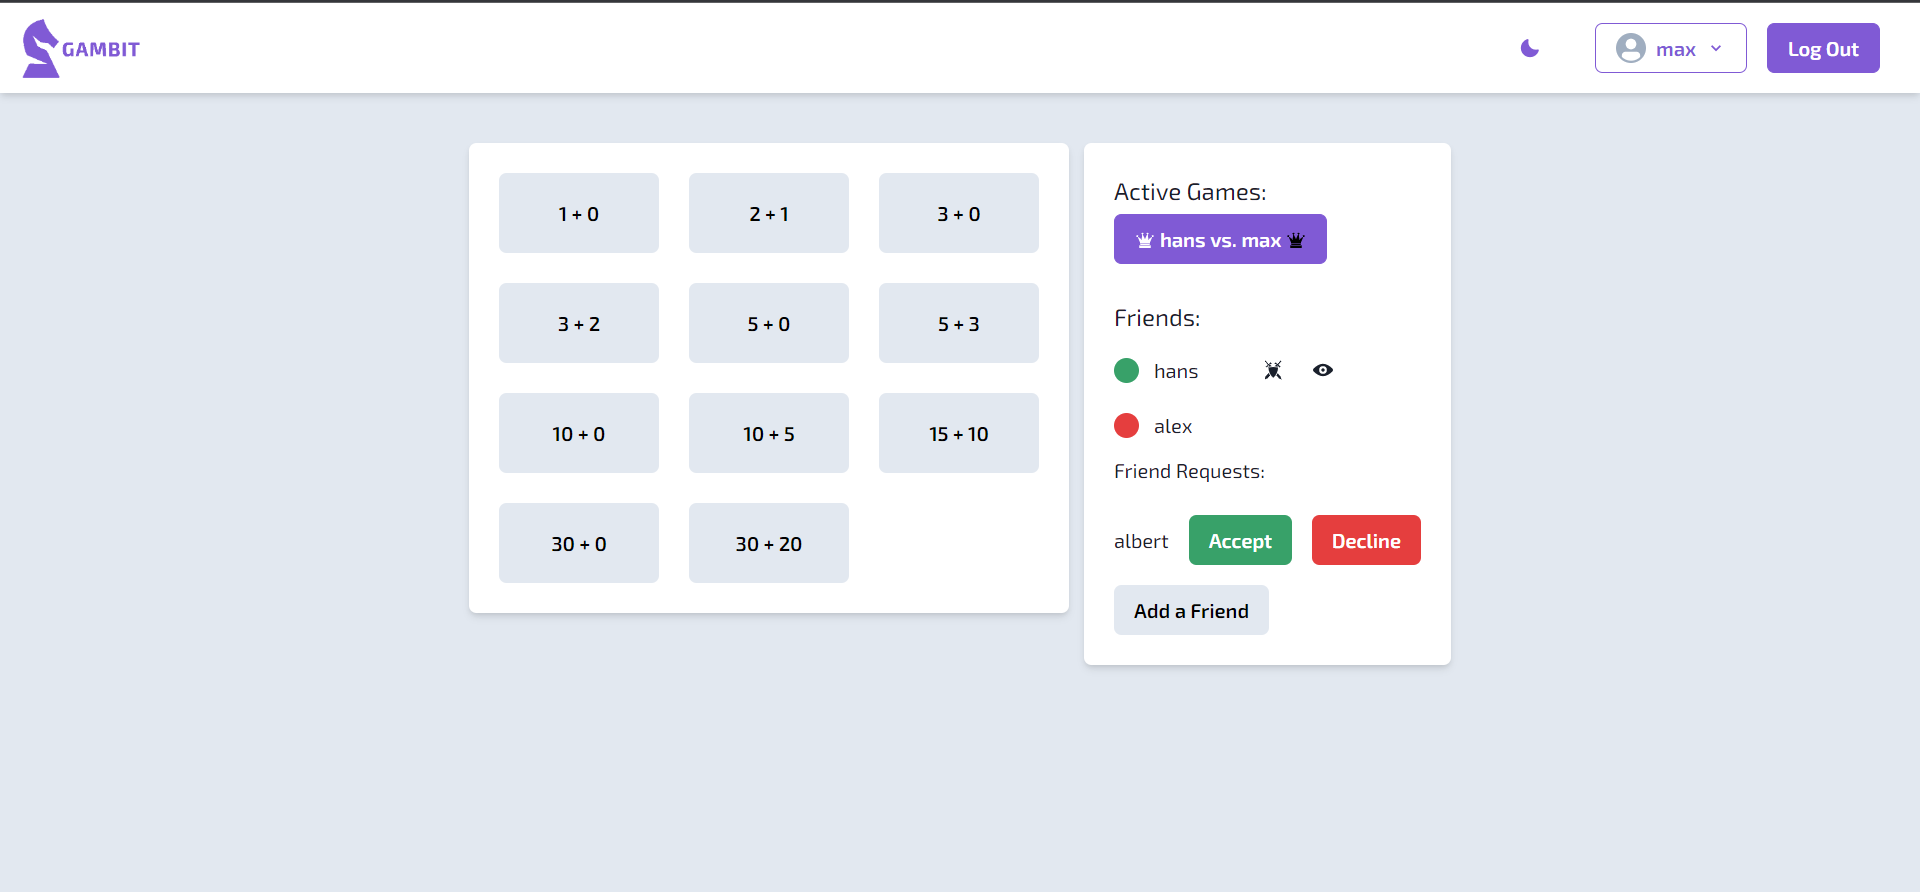
\includegraphics[width=160mm]{Home_logged_in.png}
  \caption{Home und Navbar Komponente eines angemeldeten Benutzers im hellen Farbschema}
  \label{fig:home-logged-in}
\end{figure}

      \begin{figure}[htbp]
      \centering
  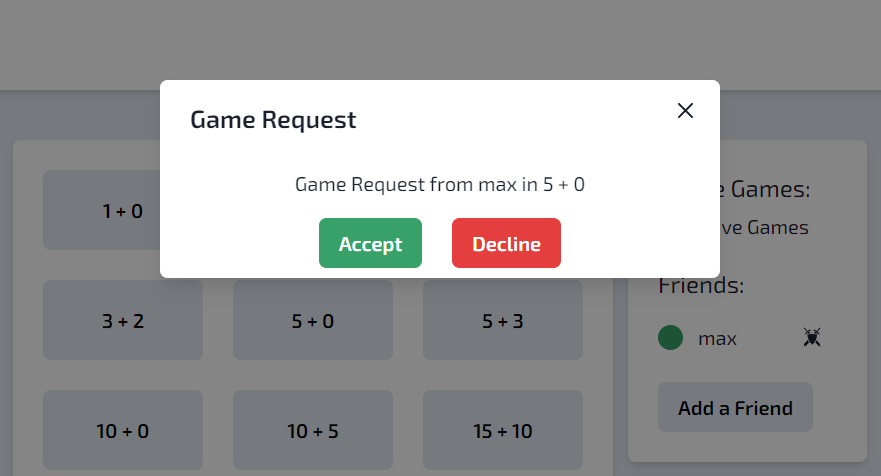
\includegraphics[width=100mm]{game_request.png}
  \caption{Das Modal der Komponente GameRequest in hellem Farbschema}
  \label{fig:game-request}
\end{figure}

      \begin{figure}[htbp]
      \centering
  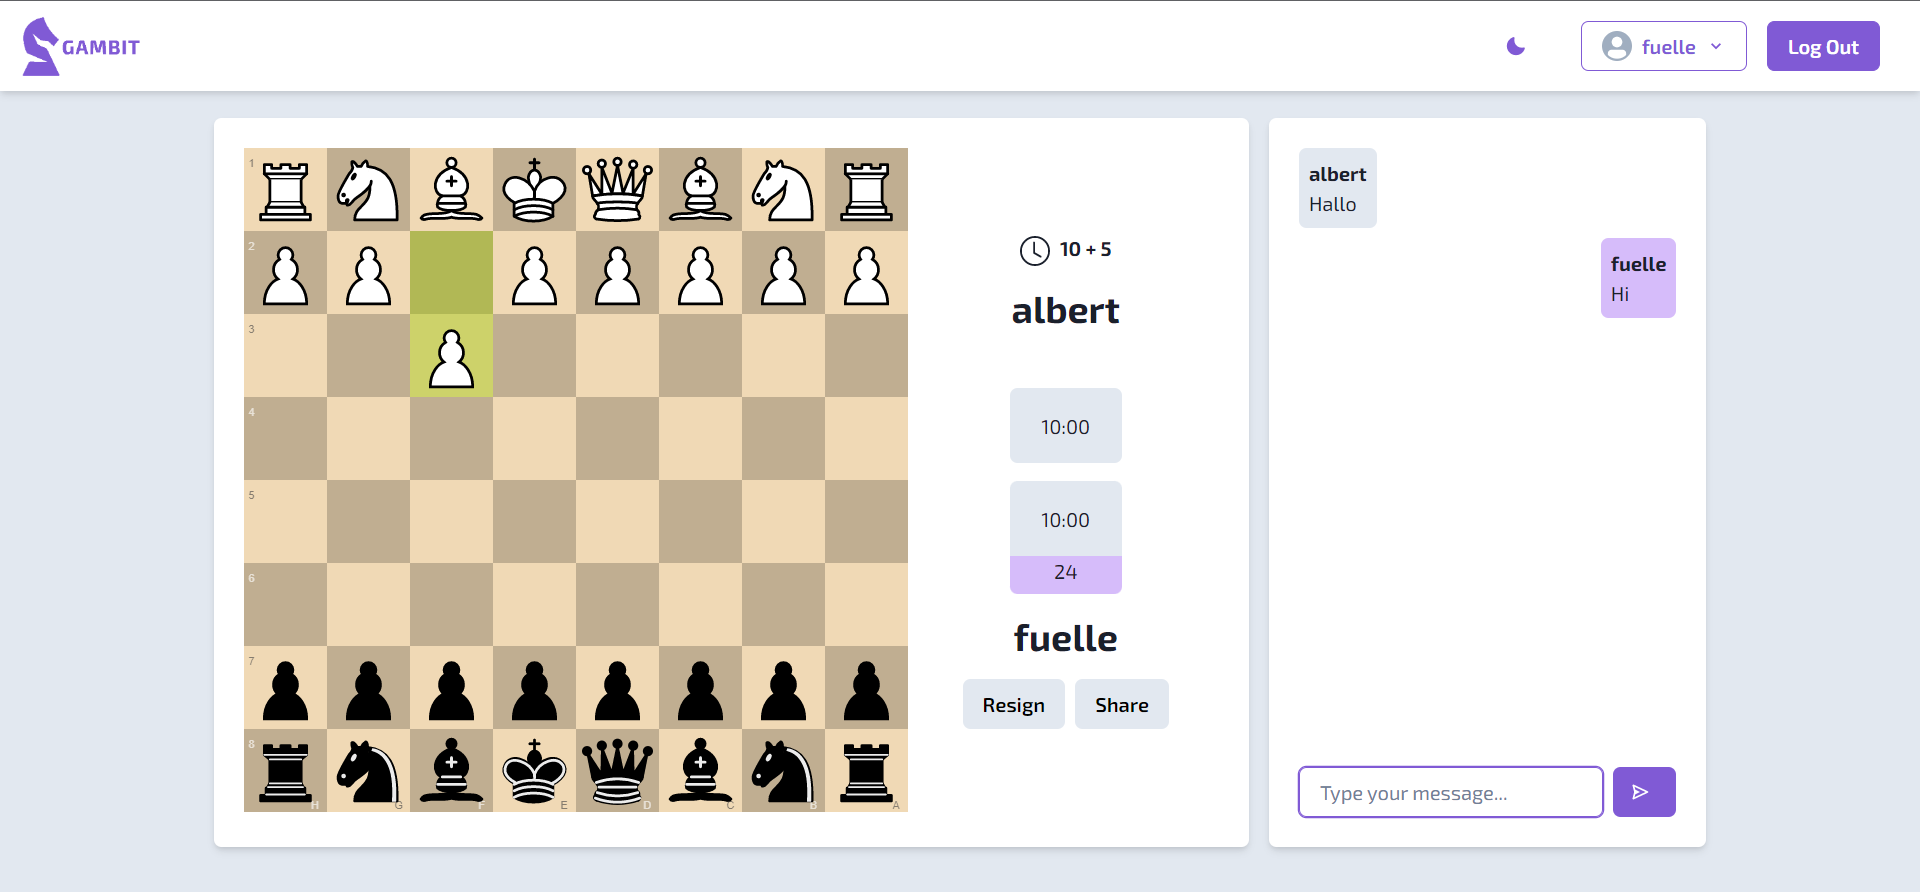
\includegraphics[width=160mm]{ChessGame.png}
  \caption{Beispiel einer ChessGame-Komponente}
  \label{fig:chess-game}
\end{figure}
        

    
   
        
        
        \subsection{Das Schachspiel}
        \label{sec:Schachspiel}
Das Schachspiel und die zugehörigen Schach Uhren sind getrennt gehalten um die Modularität zu erhöhen. Die Schachuhren und das Spiel haben jeweils eigene Events und Listener auf die sie hören.

In diesem Kapitel werde ich näher darauf eingehen wie das Schachspiel im Frontend verwaltet und aktualisiert wird. Die Vorgehensweise im Backend und im Zusammenspiel finden Sie //REFERENZ
        \subsubsection{Das Spiel}
Das Schachspiel findet in der Komponente \textit{ChessGame} statt.
Nach dem rendern der Komponente wird das \verb|get_game_data| Event mit der roomId des Spiels und einer Callback Methode gesendet, die die Daten des Spiels beinhaltet, falls dieses existiert. Falls diese Partie nicht im Backend existiert, also keine Daten gesendet werden, wird der Benutzer darauf hingewiesen.

Die Daten die gesendet werden umfassen folgendes:
\begin{itemize}
\item Der Namen des weißen und des schwarzen Spielers.
\item Welcher Zeitmodus gespielt wird (z.B.: 5 + 3, 10 + 5, ...)
\item Die aktuelle Stellung der Partie
\item Die bisherigen Nachrichten im Chat.
\item Die aktuelle Phase des Spiels: Dabei gibt es die vier Möglichkeiten, dass die Startzeit von Schwarz oder Weiß läuft oder dass die reguläre Zeit von Schwarz oder Weiß läuft.
\item Die aktuellen Zeiten der Spieler.
\end{itemize}
Diese Informationen werden für den Fall benötigt, dass man die Seite neu lädt, über die \verb|ActiveGames|-Komponente auf die Seite gelangt, über einen Link der Partie beitritt oder ähnliches. Das Einholen dieser Daten gewährleistet, dass man auch in diesen Fällen noch ohne Veränderungen weiterspielen kann.

Aufgrund der gesendeten Namen der Spieler wird definiert, ob man ein Zuschauer oder ein Spieler ist und wie das Schachbrett, die Namen und die Schachuhren ausgerichtet sind. Ist man Zuschauer wird in chessground definiert, dass man keine Figuren bewegen darf und es gibt kein input Feld für den Chat, welches verhindert, dass man Nachricht versenden kann.

Zum Spielen der Partie werden folgende Listener definiert:
\begin{itemize}
\item \verb|opponent_move|: Dient zu Empfangen eines Zugs eines Spielers.
\item \verb|checkmate|: Ein Event welches bei Schachmatt mit dem Benutzernamen des Gewinners empfangen wird.
\item \verb|time_over|: Ist eine Benachrichtigung, dass die Zeit eines Spielers abgelaufen ist.
\item \verb|draw|: Kommuniziert ein Patt der Partie.
\item \verb|resigned|: Signalisiert, dass ein Spieler aufgegeben hat.
\item \verb|cancel_game|: Das Spiel wird aufgrund der abgalaufenen Start Zeit abgebrochen.
\end{itemize}
Die Events \verb|checkmate|, \verb|time_over|, \verb|draw|, \verb|resigned| und \verb|cancel_game| beschreiben alle das Ende des Schachspiels. In ihren Listenern wird definiert, dass man keine Figur des Schach Interfaces von chessground mehr bewegen darf und man wird über den Ausgang des Spiels in Form von einem Toast benachrichtigt. //BILD

Der Ablauf beim Empfangen eines neuen Zugs ist im Aktivitätsdiagramm in Abbildung \ref{fig:chess-opponent-move} dargestellt. Die Bauernumwandlung und das En Passant müssen separat behandelt werden, da chessground nur das Schach Interface zur Verfügung stellt und bei diesen beiden Zusatzregeln andere Figuren ersetzt oder entfernt werden, als bei regulären Zügen. Das aktualisieren möglicher Züge beinhaltet, dass chessground alle möglichen Züge von chess.js übertragen bekommt, welches zur Folge hat, dass bei einem Klick auf eine Figur korrekt angezeigt wird wohin diese Figur ziehen könnte und auch nur auf diese Felder kann eine Figur dann bewegt werden (siehe Abbildung \ref{fig:chess-game}).

Gesendet werden können diese Events: \verb|new_move| zum senden eines Zugs, \verb|resign| zum Aufgaben der Partie und \verb|leave_room|, wenn der Spieler die \textit{ChessGame} Komponente verlässt.
Ein Aktivitätsdiagramm des Senden eines Zugs befindet sich in Abbildung \ref{fig:chess-move}. Genau wie bei dem Empfangen eines Zugs wird auch beim Senden zwischen Bauernumwandlung und En Passant unterschieden. Der einzige Unterschied ist, dass bei der Bauernumwandlung nach dem setzen des Zuges noch mittels des  \textit{PromotionModal} ausgewählt werden muss, in welche Figur sich der Bauer umwandeln soll, bevor der Zug gesendet wird.

Das Event zum Aufgeben wird nach dem klicken des \glqq resign\grqq{ }Buttons gesendet.


      \begin{figure}[h]
      \centering
  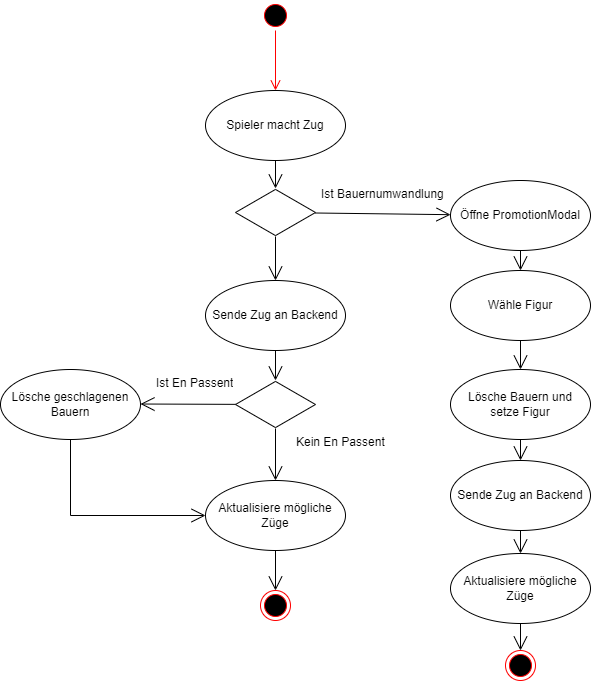
\includegraphics[width=120mm]{Interaktion Schach Zug.png}
  \caption{Aktivitätsdiagramm eines Schach Zugs}
  \label{fig:chess-move}
\end{figure}

      \begin{figure}[h]
      \centering
  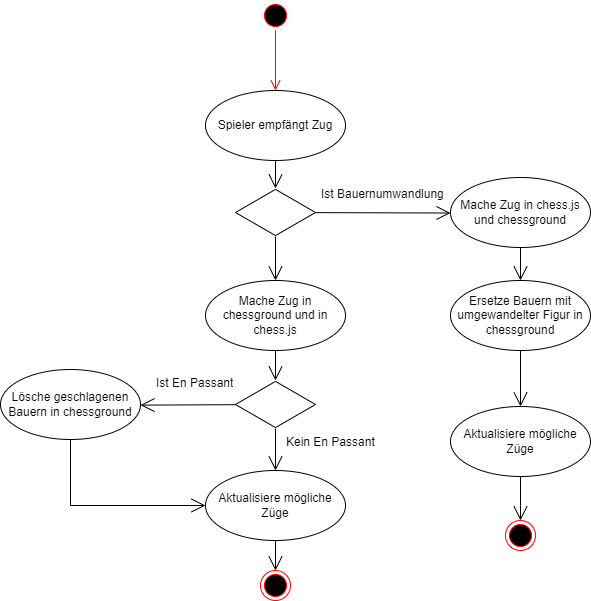
\includegraphics[width=120mm]{Interaktion Schach Zug empfangen.png}
  \caption{Aktivitätsdiagramm eines empfangenen Schach Zugs}
  \label{fig:chess-opponent-move}
\end{figure}

        \subsubsection{Die Uhr}
Die \textit{ChessClock} Komponente bekommt von \textit{ChessGame} als Props die aktuelle Phase der Partie, die jeweiligen aktuellen Zeiten und die Ausrichtung, welche Zeit oben bzw. unten gezeigt werden soll.

Die Komponente sendet keine Events, sondern hört nur auf die folgenden:
\begin{itemize}
\item \verb|updated_time|: Dieses Event wird vom Backend gesendet, sobald ein Zug gemacht wurde und enthält die aktuellen Zeiten der Spieler nach dem Zug und welcher Spieler jetzt am Zug ist. Dementsprechend werden die Zeiten aktualisiert und die Uhr des Spielers, welcher jetzt dran ist wird gestartet.
\item \verb|stop_starting_time_white|: Stoppt die Start Zeit des weißen Spielers und startet die Start Zeit des schwarzen Spielers.
\item \verb|stop_starting_time_black|: Stoppt die Start Zeit des schwarzen Spielers und lässt die reguläre Zeit des weißen Spielers beginnen.
\item \verb|stop_clocks|: Wird bei Beendung des Spiels empfangen und stoppt die aktive Uhr.
\end{itemize}

    
        \section{Backend-Architektur}
Das Backend basiert auf Node.js mit dem Express Framework. Des weiteren werden als Schnittstellen mit dem Frontend eine Web-API für HTTP Anfragen und ein Socket.io Server bereitgestellt. Das Backend kommuniziert mit zwei Datenbanken: einer PostgreSQL Datenbank für die Benutzerverwaltung und eine Redis Datenbank für häufig aktualisierte und angefragte Daten.

Die Ordnerstruktur des Backends (Abbildung \ref{fig:backend_dirtree}) ist auf dieser Weise aufgebaut:

\begin{itemize}
\item \textbf{auth:} Dieser Ordner beschäftigt sich sowohl mit der Schnittstelle der Web-API Kommunikation mit dem Frontend, als auch deren Behandlung und dem Austausch mit der PostgreSQL Datenbank. Diese Schnittstellen dienen bloß der Anmeldung und Registrierung eines Benutzers.
\item \textbf{chess:} Stellt ein chess.js Schachspiel zur Verfügung und die serverseitige Schachuhr.
\item \textbf{redis:} Dient als Schnittstelle und Verwalter von Operationen auf der redis Datenbank.
\item \textbf{sockets:} Stellt Middleware für die Verbindungsherstellung und Listener für die Kommunikation zwischen Frontend und Backend bereit.
\item \textbf{index.js:} Initialisiert den Server mit seinen Schnittstellen.
\end{itemize}

\begin{figure}[h]
\centering

\begin{minipage}{0.6\textwidth}
\dirtree{%
.1 server/.
.2 src/.
.3 auth/ .
.4 authController.js.
.4 database.js.
.4 rateLimiter.js.
.4 validateForm.js.
.3 chess/.
.4 Chess.mjs.
.4 ServerChessClock.js.
.3 redis/.
.4 redis.js.
.4 redisController.js.
.3 routers/.
.4 authRouter.js.
.3 sockets/.
.4 socketChessController.js.
.4 socketController.js.
.4 socketMiddleware.js.
.2 .env.
.2 index.js.
.2 package.json.
}
\end{minipage}
\caption{Ordnerstruktur des Backends}
\label{fig:backend_dirtree}

\end{figure}


\subsection{Authentifizierung}
Die Authentifizierung eines Benutzers läuft über HTTP Anfragen an der Web-API und einer PostgreSQL Datenbank.
Nachdem die erste Authentifizierung stattgefunden hat wird die Socket.io Verbindung des Clients hergestellt, in der der Benutzer nochmals Authentifiziert wird.
Es gibt drei verschiedene Möglichkeiten wie ein Benutzer authentifiziert werden kann: Durch das Anmelden, durch das Registrieren oder durch das Lesen des Cookies beim Aufruf der Seite vom Client.

\subsubsection{Authentifizierung mit der Web-API und PostgreSQL}
Das Anmelden und Registrieren mittels Formular läuft über eine POST Anfrage des Clients an den Pfad \verb|/auth/login|, beziehungsweise \verb|/auth/signup|, die die angegebenen Formulardaten beinhaltet. Bei der Verarbeitung der Anfrage werden mittels des Express Routing verschiedene Middlewares verwendet.

Eine Middleware stellt sicher, dass die Anzahl der Anfragen über eine IP-Adresse in einer bestimmten Zeit begrenzt wird. Dies verhindert sogenannte Denial-of-Service (kurz: DoS) Attacken\footnote{Quelle: \url{https://www.bsi.bund.de/DE/Themen/Verbraucherinnen-und-Verbraucher/Cyber-Sicherheitslage/Methoden-der-Cyber-Kriminalitaet/DoS-Denial-of-Service/dos-denial-of-service_node.html} am 27. April 2023}, bei denen probiert wird den Server mit so vielen Anfragen zu belasten, dass dieser außer Betrieb gesetzt wird.

Anschließend überprüft eine Middleware, ob die angegebenen Daten mit dem Schema übereinstimmen. 

Treten bei diesen beiden Middlewares keine Fehler auf wird beim Anmelden überprüft, ob dieser Benutzer in der Datenbank existiert und es wird mittels bcrypt überprüft ob die Passwörter übereinstimmen. Ist dies der Fall, wird ein JWT-Token mit den Benutzerinformationen erstellt und als Cookie in den Browser des Clients gesetzt. Des weiteren wird dem Benutzer natürlich geantwortet, dass die Anmeldung erfolgreich war.

Beim Registrieren wird überprüft, ob bereits ein Nutzer mit dem Benutzernamen oder E-Mail existiert und anschließend wird ein neuer Tupel in der PostgreSQL Datenbank erstellt, der Cookie mit dem JWT-Token gesetzt und dem Benutzer geantwortet.

Bei dem ersten Aufruf der Seite vom Client wird eine GET Anfrage an \verb|/auth/login| gestellt. Bei dieser wird ebenfalls die Middleware gegen DoS-Attacken verwendet und anschließend wird überprüft, ob er einen gültigen JWT-Token im Cookie hat und ihm wird dem entsprechend geantwortet. Das setzen des Tokens im Cookie hat den Vorteil, dass beim neuen Aufruf der Seite, solange der Cookie noch gültig ist, der Benutzer automatisch angemeldet ist, ohne seine Anmeldedaten nochmals einzugeben.

Anschließend stellt der Client eine Socket.io Verbindung her.

\subsubsection{Authentifizierung und anschließende Middleware mit Socket.io}
Bei der Verbindungsherstellung des Clients mit dem Socket.io Server durchläuft die socket verschiedene Middlewares.

Die erste Middleware Authentifiziert die Socket des Benutzer. Sie liest aus dem Cookie, der auch in der socket mitgesendet wird, den JWT-Token, falls dieser existiert. Die Daten die in dem Token kodiert sind werden dann in der Socket als Attribute gesetzt, sodass anschließend immer mittels \verb|socket.user| darauf zugegriffen werden kann.

Wenn der Benutzer keinen gültigen JWT-Token hat, werden trotzdem alle Middlewares ohne Fehler durchlaufen. Dies liegt daran, dass bei einem fehlgeschlagenen Middleware-Prozess die Socket.io-Verbindung abgelehnt werden würde. Es soll allerdings auch das Spielen einer Schachpartie als Gast möglich sein.

Als zweite Middleware wird der Benutzer mit Daten versorgt, er tritt dem Raum seiner userid bei und wird als online vermerkt. Dabei wird in Redis \verb|user:username| mit seinen Informationen und \verb|connected true| gesetzt. Anschließend werden alle Freunde des Benutzers aus der Redis Datenbank geholt und an alle ein Event gesendet, das signalisiert, dass der Benutzer online ist. Des weiteren werden auch Informationen bezüglich aktiver Spiele und Freundschaftsanfragen aus Redis abgerufen und mittels entsprechenden Events werden die Informationen über Freunde, aktive Partien und Freundschaftsanfragen an den Benutzer gesendet.

Als letzte Middleware werden alle nötigen Listener sowohl für das Schachspiel, als auch für sonstige Funktionen initialisiert.


		\section{Datenbankstruktur}
\subsection{PostgreSQL Datenbank}
Die PostgreSQL Datenbank wird ausschließlich für die Anmeldung und Registrierung genutzt. Sie enthält eine Tabelle mit folgendem Schema:
\begin{itemize}
\item \textbf{id:} Eine Fortlaufende id, die als Primärschlüssel dient.
\item \textbf{email:} Die E-Mail, die bei der Registrierung angegeben wurde.
\item \textbf{username:} Der Benutzername des Benutzers.
\item \textbf{userid:} Jeder Spieler erhält beim Registrieren seine eigene userid. Diese dient der Kommunikation mit dem Benutzer. Bei einer Verbindung mit Socket.io erhält die socket immer eine andere Id, also wie sendet man ein Event an einen bestimmten Spieler? Diese userid löst das Problem, indem man nach dem anmelden immer dieser id als Raum beitritt. Somit kann immer an diese Id gesendet werden und man stellt sicher, dass der Client das Event empfängt.
\item \textbf{password:} Das mit bcrypt verschlüsselte Passwort des Benutzers.
\end{itemize}
Jedes dieser Attribute, außer das Passwort, hat die Einschränkung, dass es einzigartig sein muss. Die E-Mail wird bisher nicht genutzt, kann aber in Zukunft zum Bestätigen der Registrierung oder Einrichtung eines Newsletters genutzt werden.

\subsection{Redis}
\subsubsection{user:username}
Unter dem Key \verb|user:username| (wobei hier \verb|username| mit dem entsprechenden Benutzernamen ausgetauscht wird) befindet sich ein Redis Hash. Ein Redis Hash besitzt Key-Value Paare, auf welche man zugreifen kann.

In unserem Fall werden folgende Values zu den Keys dort gespeichert:
\begin{itemize}
\item \textbf{userid:} Auch hier wird die userid gespeichert, da Redis vor allem für socket.io Funktionen verwendet wird und daher eine kurze Abfragezeit benötigt.
\item \textbf{connected:} Ist \glqq true\grqq{ } oder \glqq false\grqq , je nachdem ob der Benutzer gerade online ist oder nicht.
\end{itemize}

\subsubsection{game:roomId}
Der Redis Hash \verb|game:roomId| verwaltet die Daten einer Schachpartie. Dazu gehören:
\begin{itemize}
\item \textbf{whitePlayer, blackPlayer:} Benutzernamen des weißen und schwarzen Spielers.
\item \textbf{time:} Der Zeitmodus welcher gespielt wird (z.B.: 15 + 10, 5 + 3, ...)
\item \textbf{pgn:} Die Historie aller bisherigen Züge im PGN Format.
\item \textbf{chat:} Alle bisher geschriebenen Nachrichten im Chat.
\end{itemize}

\subsubsection{activeGames:username}
\verb|activeGames:username| beinhaltet eine Liste der aktiven Spiele dieses Benutzers. In der Liste stehen alle roomIds der aktiven Spiele.

\subsubsection{friends:username}
Der Key \verb|friends:username| verweist auf eine Liste von Freunden. Diese Freunde bestehen aus einem String, der sich zusammensetzt aus username:userid. Dies verhindert, dass wenn man ein Event an einen Freund senden will, man einen extra Zugriff auf user:username machen muss um die userid zu bekommen.

\subsubsection{friend\_requests:username}
Dies ist eine Liste die genauso aufgebaut ist wie die \verb|friends:username| Liste, außer, dass sie Freundschaftsanfragen verwaltet.

\subsubsection{Warteschlangen}
\label{sec:Warteschlange}
Die letzten Elemente sind die Warteschlangen für Spiele. Diese bestehen aus \verb|waitingPlayers:timeMode| und \verb|waitingGuests:timeMode|, je nachdem, ob es sich um einen angemeldeten Benutzer handelt oder nicht. \verb|timeMode| repräsentiert hier alle möglichen Schachuhren, also beispielsweise \glqq 10 + 5\grqq , \glqq 15 + 10\grqq , ...

Diese Warteschlagen sind Listen, welche aus \verb|username:userid| Einträgen bestehen, um die Anzahl an Abfragen zu verringern. 

Durch die Redis Operationen \verb|RPOP| und \verb|LPUSH| lassen sich atomar Einträge hinzufügen oder herausnehmen, welches die Konsistenz der Liste gewährleistet.
        \section{Interaktion zwischen Frontend und Backend}
Es gibt einige Funktionen die nur durch komplexere Interaktionen zwischen Frontend, Backend und Datenbank möglich sind. Um diese Interaktionen besser zu verstehen werde ich sie in diesem Kapitel mittels Sequenzdiagrammen erläutern.

\subsection{Suchen einer Partie mit unbekanntem Gegner}
\label{sec:game-suche}
Um eine Schachpartie mit einem zufälligen Gegner zu starten klickt man auf einen der Buttons mit den Zeitkonfigurationen in der \textit{Home}-Komponente (siehe Abbildung \ref{fig:home-not-logged-in} oder \ref{fig:home-logged-in}). Der Ablauf, wie ein Spieler gefunden wird und ein Spiel gestartet wird werde ich hier erklären. In Abbildung \ref{fig:sequence_chess_start} ist ein Sequenzdiagramm dieses Ablaufs dargestellt.

\begin{itemize}
\item Sobald ein Spieler auf einen der Buttons klickt, wird das Event \verb|find_game| mit der Zeitkonfiguration gesendet.
\item Falls der Benutzer nicht angemeldet ist, wird ihm  ein zufälliger username zugewiesen, der mit \glqq guest-\grqq{ }startet. Seine userid wird als seine socket id festgelegt.
\item Daraufhin wird im Server ein Spieler aus der entsprechenden Warteschlange aus Redis genommen (siehe Abschnitt \ref{sec:Warteschlange}).
\item Falls dabei kein Spieler entnommen werden konnte, wird der Benutzer selbst in die Liste geschrieben und wartet bis er von einem anderen Benutzer aus der Liste genommen wird.
\item Falls ein Spieler aus der Liste entnommen werden konnte, wird das Spiel mit einer \textit{roomId} als Identifikator initialisiert und in Redis gespeichert.
\item An die beiden Spieler wird das Event \verb|joined_game| mit der roomId gesendet, woraufhin sie zu dem Pfad \verb|/game/roomId| navigieren, auf der sich die \textit{ChessGame}-Komponente befindet.
\item Die \textit{ChessGame}-Komponente sendet das \verb|get_game_data| Event. Daraufhin wird der aktuelle Zustands der Partie aus Redis geholt und an das Frontend zurück gesendet. Ein Ablauf was im Frontend bei einer Schachpartie passiert befindet sich im Abschnitt \ref{sec:Schachspiel}.
\end{itemize}
      
        
\begin{figure}
  \centering
  
  \begin{sequencediagram}[scale=0.2]
    \newinst{clientA}{Client A}
    \newinst[2]{clientB}{Client B}
    \newthread{server}{Server}
    \tikzstyle {inststyle}+=[rounded corners=3mm]
    \newinst[3]{redis}{Redis DB}
    
    \begin{messcall}{clientA}{find\_game}{server}
    \begin{call}{server}{getPlayerInQueue}{redis}{player}
    \end{call}
    
    \begin{sdblock}{Kein Spieler in der Warteschlange}{}
    	\begin{messcall}{server}{addPlayerInQueue}{redis}{}
    	\end{messcall}
    	\end{sdblock}
    	
    	\begin{messcall}{clientB}{find\_game}{server}{}
    	\end{messcall}
    	
    \begin{call}{server}{getPlayerInQueue}{redis}{player}
    \end{call}
    	
    	\begin{sdblock}{Spieler in Warteschlange}{}
    \begin{callself}{server}{Erstelle Spiel}{roomId}
    \end{callself}
    \postlevel
    	\begin{messcall}{server}{Speichere Spiel}{redis}
    	\end{messcall}
    	\prelevel
    	\begin{messcall}{server}{joined\_game, roomId}{clientA}{}
    	\prelevel\prelevel
    	\mess{clientA}{navigiere zu /game/roomId}{clientA}
    	\postlevel\postlevel
    	\begin{call}{clientA}{get\_game\_data, roomId}{server}{gameData}
    	\begin{call}{server}{Hole Daten des Spiels}{redis}{gameData}
    	\end{call}
    	\end{call}
    	\end{messcall}
    	\prelevel
    	\begin{messcall}{server}{}{clientB}{}
    	\begin{call}{clientB}{}{server}{}
    	\begin{call}{server}{}{redis}{}
    	\end{call}
    	\end{call}
    	\end{messcall}
    	\end{sdblock}
    \end{messcall}
    
    
    
  \end{sequencediagram}
  \caption{Sequenzdiagramm des Schachspielstartprozesses mit unbekanntem Gegner}
  \label{fig:sequence_chess_start}
\end{figure}

